\section{Further experimental details and results}
\label{sec:exp_details}

\subsection{Bayesian neural network}
We detail the experimental set-up of the Bayesian neural network example.
%
For regression tests, we consider Protein and Year as the large datasets and the others as small datasets. The likelihood function is defined as $p(y|\bm{x}, \bm{\theta}) = \mathcal{N}(y; F_{\bm{\theta}}(\bm{x}), \sigma^2)$ where $F_{\bm{\theta}}(\bm{x})$ denotes the non-linear transform from the neural network with weights $\bm{\theta}$. We use unit Gaussian prior $\bm{\theta} \sim \mathcal{N}(\bm{\theta}; \bm{0}, \bm{I})$ and Gaussian approximation $q(\bm{\theta}) = \mathcal{N}(\bm{\theta}; \bm{\mu}_q, diag(\bm{\sigma}_q))$, where we fit the parameters of $q$ and the noise level $\sigma$ by optimising the lower-bound. For all datasets we use single-layer neural networks with 50 hidden units (ReLUs) for datasets except Protein and Year (100 units). The methods for comparison were run for $500$ epochs on the small datasets and $100$, $40$ epochs for the large datasets Protein and Year, respectively. We used ADAM \cite{kingma:adam} for optimisation with learning rate 0.001 and the standard setting for other parameters. For stochastic optimisation we used learning rate $0.001$, mini-batch size $M = 32$ and number of samples $K=100, 10$ for small and large datasets. The number of dataset random splits is 20 except for the large datasets, which is 5 and 1 for Protein and Year, respectively. 

The full test results are provided in Figure \ref{fig:bnn_results_all} and Table \ref{tab:bnn_ll}, \ref{tab:bnn_rmse}. In the tables the best performing results are underlined, while the worse cases are also bold-faced. Clearly the optimal $\alpha$ setting is dataset dependent, although for Boston and Power the performances are very similar. Also for Naval mass-covering seems to be harmful not only for predictive error but also for test log-likelihood measure. Overall mode-seeking methods tend to focus on improving the predictive error, while mass-covering regimes often return better test log-likelihood. 


\subsection{Variational auto-encoder}
We describe the network architecture tested in the VAE experiments. The number of stochastic layers $L$, number of hidden units, and the activation function are summarised in Table \ref{tab:vae_arch}. The prefix of the number indicates whether this layer is \textbf{d}eterministic or \textbf{s}tochastic, e.g.~d500-s200 stands for a neural network with one deterministic layer of 500 units followed by a stochastic layer of 200 units. For Frey Face data we train the models using learning rate 0.0005 and mini-batch size 100. For MNIST and OMNIGLOT we reuse the settings from \cite{burda:iwae}: the training process runs for $3^i$ passes with learning rate $0.0001 \cdot 10^{-i/7}$ for $i = 0, ..., 7$, and the batch size is 20. For Caltech Silhouettes we use the same settings as MNIST and OMNIGLOT except that the training proceeded for $\sum_{i=0}^7 2^i = 255$ epochs.

We also present some samples from the VR-max trained auto-encoders in Figure \ref{fig:vae_samples}, and note that the visual quality of these samples are almost identical to those from IWAE.

\begin{figure}[ht]
\centering
    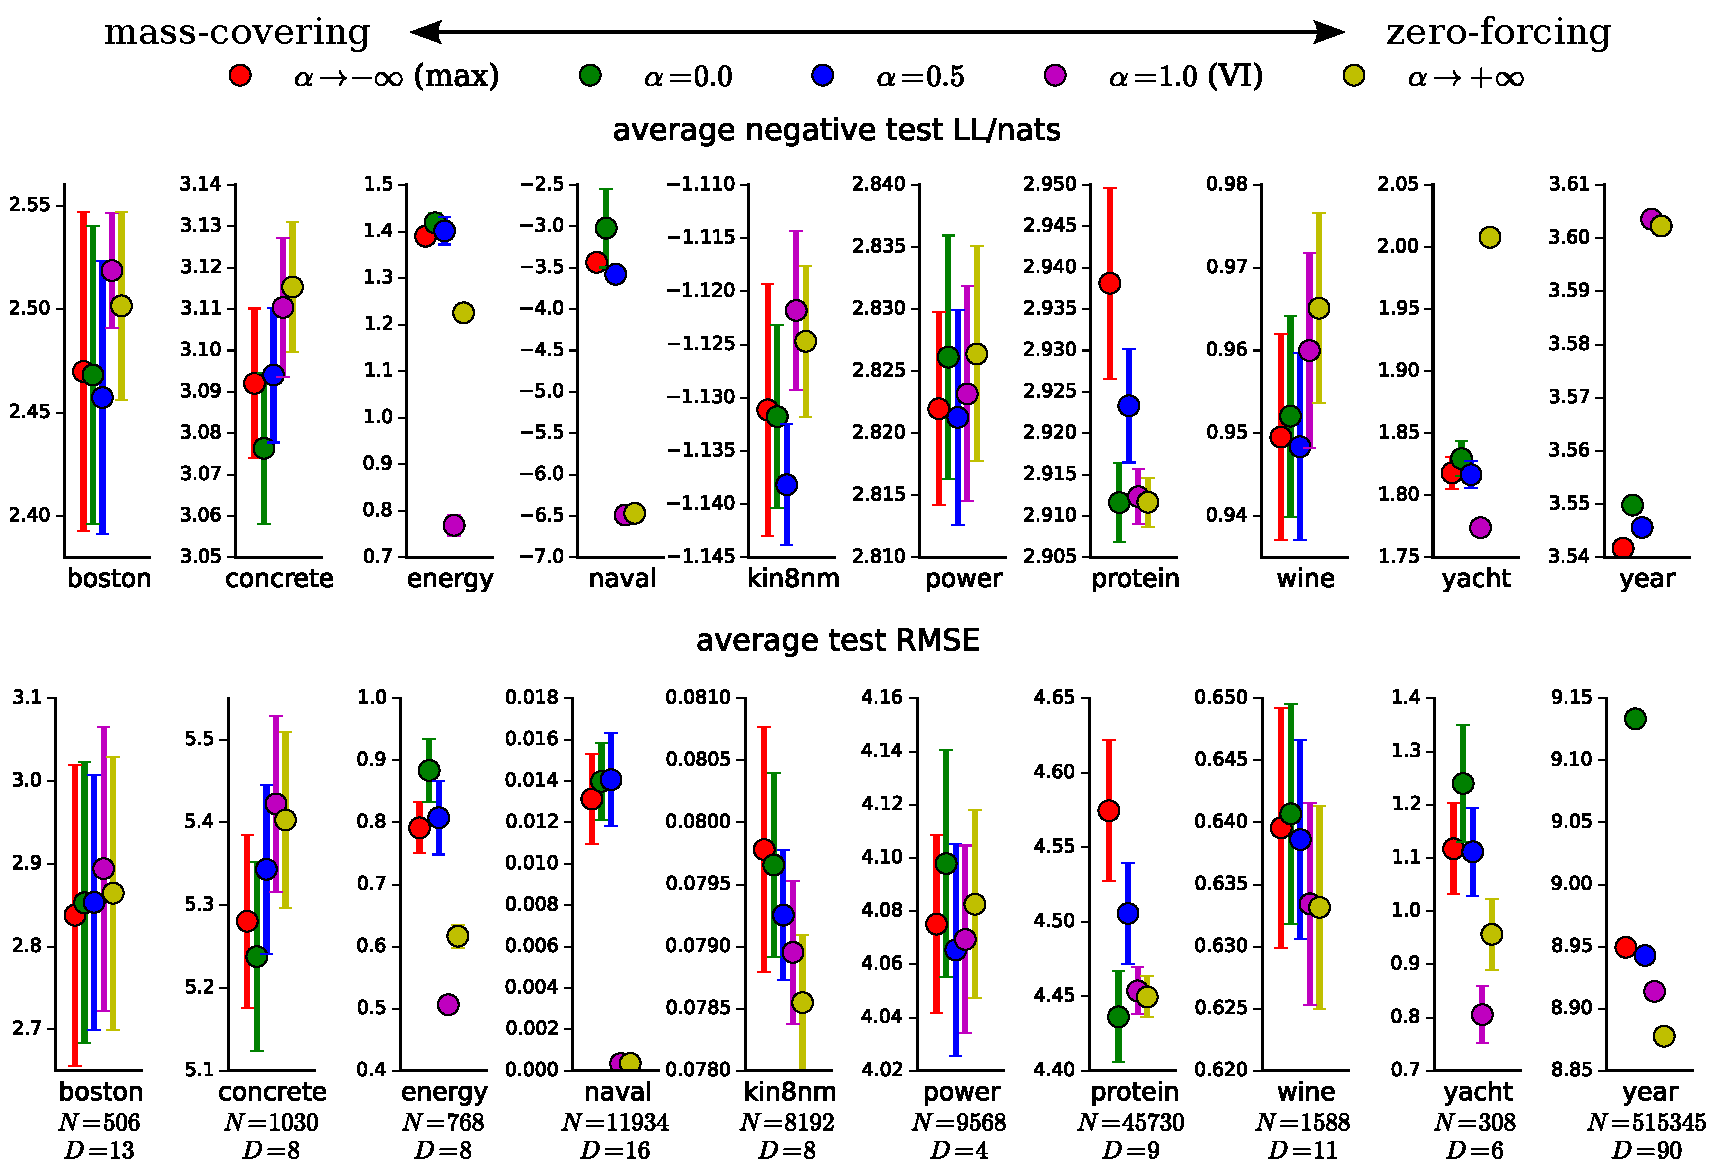
\includegraphics[width=1\linewidth]{../figs/results_all_bnn.pdf}
    \caption{Test LL and RMSE results for Bayesian neural network regression. The lower the better.}
    \label{fig:bnn_results_all}

%\begin{table}[ht]
\centering
\captionof{table}{Regression experiment: Average negative test log likelihood/nats}
\label{tab:bnn_ll}
\begin{tabular}{l@{\ica}r@{\ica}r@{\ica}r@{$\pm$}l@{\ica}r@{$\pm$}l@{\ica}r@{$\pm$}l@{\ica}r@{$\pm$}l@{\ica}r@{$\pm$}l@{\ica}}
\hline
\bf{Dataset}&{N}&{D}&\multicolumn{2}{c}{\bf{$\alpha \rightarrow -\infty$}}&\multicolumn{2}{c}{\bf{$\alpha = 0.0$}}&\multicolumn{2}{c}{\bf{$\alpha = 0.5$}}&\multicolumn{2}{c}{\bf{$\alpha = 1.0$ (VI)}}&\multicolumn{2}{c}{\bf{$\alpha \rightarrow +\infty$}}\\
\hline
boston&506&13&2.47&0.08&2.47&0.07&\underline{\textit{2.46}}&\underline{\textit{0.07}}&\textbf{2.52}&\textbf{0.03}&2.50&0.05\\
concrete&1030&8&3.09&0.02&\underline{\textit{3.08}}&\underline{\textit{0.02}}&3.09&0.02&3.11&0.02&\textbf{3.12}&\textbf{0.02}\\
energy&768&8&1.39&0.02&\textbf{1.42}&\textbf{0.02}&1.40&0.03&\underline{\textit{0.77}}&\underline{\textit{0.02}}&1.23&0.01\\
naval&11934&16&-3.43&0.08&\textbf{-3.02}&\textbf{0.48}&-3.58&0.08&\underline{\textit{-6.49}}&\underline{\textit{0.04}}&-6.47&0.09\\
kin8nm&8192&8&-1.13&0.01&-1.13&0.01&\underline{\textit{-1.14}}&\underline{\textit{0.01}}&\textbf{-1.12}&\textbf{0.01}&-1.12&0.01\\
power&9568&4&2.82&0.01&2.83&0.01&\underline{\textit{2.82}}&\underline{\textit{0.01}}&2.82&0.01&\textbf{2.83}&\textbf{0.01}\\
protein&45730&9&\textbf{2.94}&\textbf{0.01}&\underline{\textit{2.91}}&\underline{\textit{0.00}}&2.92&0.01&2.91&0.00&2.91&0.00\\
wine&1588&11&0.95&0.01&0.95&0.01&\underline{\textit{0.95}}&\underline{\textit{0.01}}&0.96&0.01&\textbf{0.97}&\textbf{0.01}\\
yacht&308&6&1.82&0.01&1.83&0.01&1.82&0.01&\underline{\textit{1.77}}&\underline{\textit{0.01}}&\textbf{2.01}&\textbf{0.00}\\
year&515345&90&\underline{\textit{3.54}}&NA&3.55&NA&3.55&NA&\textbf{3.60}&NA&3.60&NA\\
\hline
\multicolumn{3}{c}{\textbf{Average Rank}}&2.80&0.34&3.00&0.45&\textbf{2.20}&\textbf{0.37}&3.20&0.51&3.80&0.39\\
\hline
\end{tabular}
%\end{table}

%\begin{table}[ht]
\centering
\captionof{table}{Regression experiment: Average test RMSE}
\label{tab:bnn_rmse}
\begin{tabular}{l@{\ica}r@{\ica}r@{\ica}r@{$\pm$}l@{\ica}r@{$\pm$}l@{\ica}r@{$\pm$}l@{\ica}r@{$\pm$}l@{\ica}r@{$\pm$}l@{\ica}}
\hline
\bf{Dataset}&{N}&{D}&\multicolumn{2}{c}{\bf{$\alpha \rightarrow -\infty$}}&\multicolumn{2}{c}{\bf{$\alpha = 0.0$}}&\multicolumn{2}{c}{\bf{$\alpha = 0.5$}}&\multicolumn{2}{c}{\bf{$\alpha = 1.0$ (VI)}}&\multicolumn{2}{c}{\bf{$\alpha \rightarrow +\infty$}}\\
\hline
boston&506&13&\underline{\textit{2.84}}&\underline{\textit{0.18}}&2.85&0.17&2.85&0.15&\textbf{2.89}&\textbf{0.17}&2.86&0.17\\
concrete&1030&8&5.28&0.10&\underline{\textit{5.24}}&\underline{\textit{0.11}}&5.34&0.10&\textbf{5.42}&\textbf{0.11}&5.40&0.11\\
energy&768&8&0.79&0.04&\textbf{0.88}&\textbf{0.05}&0.81&0.06&\underline{\textit{0.51}}&\underline{\textit{0.01}}&0.62&0.02\\
naval&11934&16&0.01&0.00&0.01&0.00&\textbf{0.01}&\textbf{0.00}&\underline{\textit{0.00}}&\underline{\textit{0.00}}&0.00&0.00\\
kin8nm&8192&8&\textbf{0.08}&\textbf{0.00}&0.08&0.00&0.08&0.00&0.08&0.00&\underline{\textit{0.08}}&\underline{\textit{0.00}}\\
power&9568&4&4.08&0.03&\textbf{4.10}&\textbf{0.04}&\underline{\textit{4.07}}&\underline{\textit{0.04}}&4.07&0.04&4.08&0.04\\
protein&45730&9&\textbf{4.57}&\textbf{0.05}&\underline{\textit{4.44}}&\underline{\textit{0.03}}&4.51&0.03&4.45&0.02&4.45&0.01\\
wine&1588&11&0.64&0.01&\textbf{0.64}&\textbf{0.01}&0.64&0.01&0.63&0.01&\underline{\textit{0.63}}&\underline{\textit{0.01}}\\
yacht&308&6&1.12&0.09&\textbf{1.24}&\textbf{0.11}&1.11&0.08&\underline{\textit{0.81}}&\underline{\textit{0.05}}&0.96&0.07\\
year&515345&90&8.95&NA&\textbf{9.13}&NA&8.94&NA&8.91&NA&\underline{\textit{8.88}}&NA\\
\hline
\multicolumn{3}{c}{\textbf{Average Rank}}&3.40&0.38&3.70&0.51&3.20&0.31&2.40&0.45&\textbf{2.30}&\textbf{0.38}\\
\hline
\end{tabular}
%\end{table}

       
\end{figure}

\begin{figure*}[t]
 \centering
 %\subfigure[Frey Face]{
 %\includegraphics[width=0.4\linewidth]{../figs/freyface_samples.pdf}}
 %\hspace{0.3in}
 %\subfigure[Caltech 101 Silhouettes]{
 %\includegraphics[width=0.4\linewidth]{../figs/silhouettes_samples.pdf}}
 %\hspace{0.3in}
 %\subfigure[MNIST]{
 %\includegraphics[width=0.4\linewidth]{../figs/mnist_samples.pdf}}
 %\hspace{0.3in}
 %\subfigure[OMNIGLOT]{
 %\includegraphics[width=0.4\linewidth]{../figs/omni_samples.pdf}}
 %\caption{Sampled images from the VR-max trained auto-encoders.}
 
  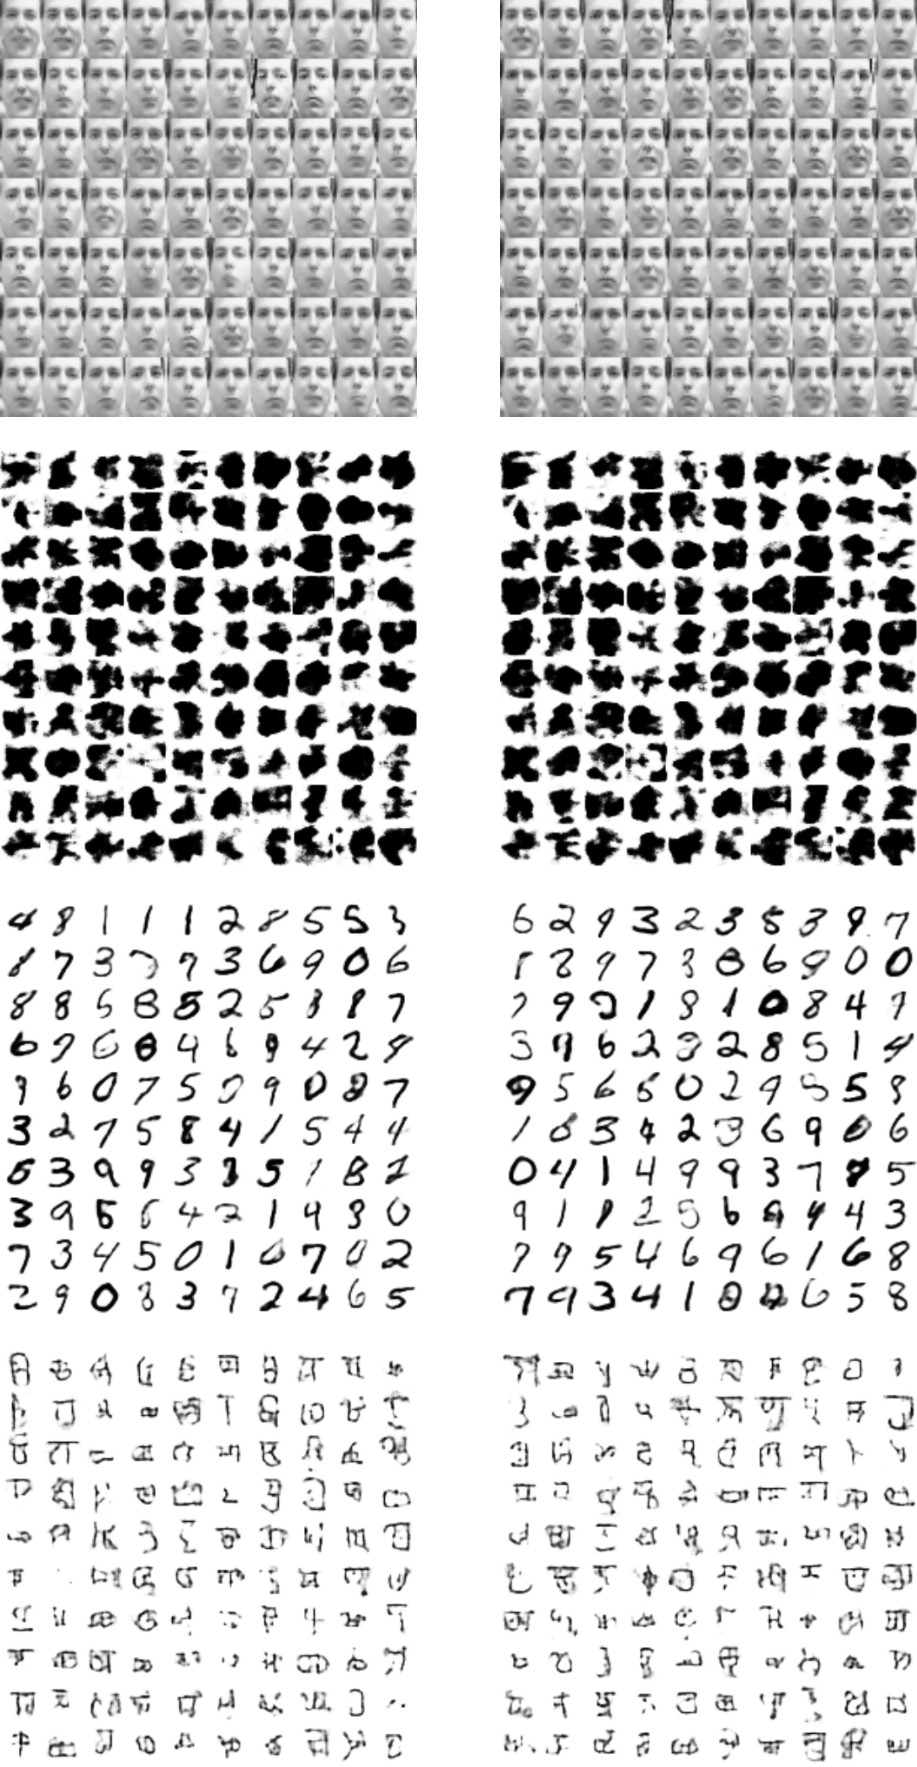
\includegraphics[width=0.6\linewidth]{../figs/vae_samples.pdf}
  \caption{Sampled images from the the best models trained with IWAE (left) and VR-max (right).}
  \label{fig:vae_samples}
%
\input{vae_architecture}
\end{figure*}